\part*{Appendix}
\addcontentsline{toc}{part}{Appendix}

\appendix

\section{555 Timer IC Circuit Diagram}
\label{app:555}
Circuit diagram of the 555 timer IC as produced by the manufacturer\cite{NE555}.
\begin{figure}[h!]
	\begin{center}
		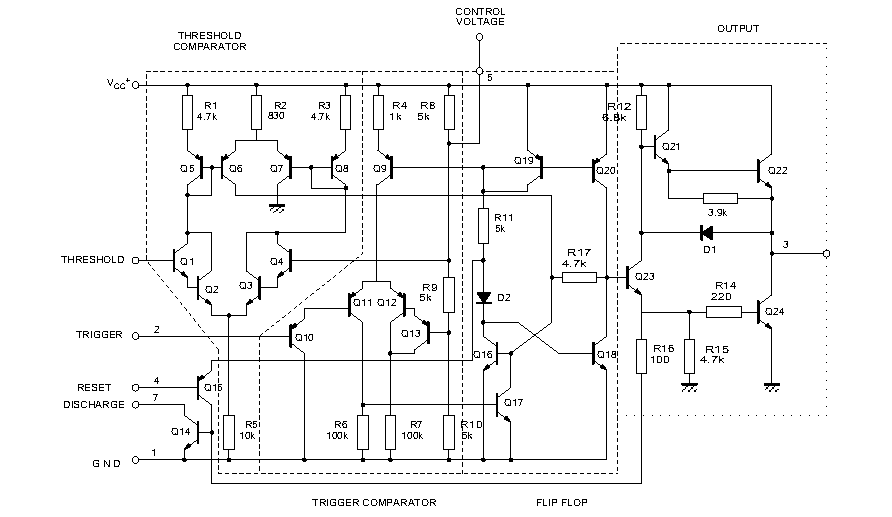
\includegraphics[scale=0.9]{report_img/555_crop}
	\end{center}
\end{figure}

\section{555 Timer IC Circuit Diagram}
\label{app:4046}
Circuit diagram of the 4046 IC as produced by the manufacturer\cite{HEF4046B}.
\begin{figure}[h!]
	\begin{center}
		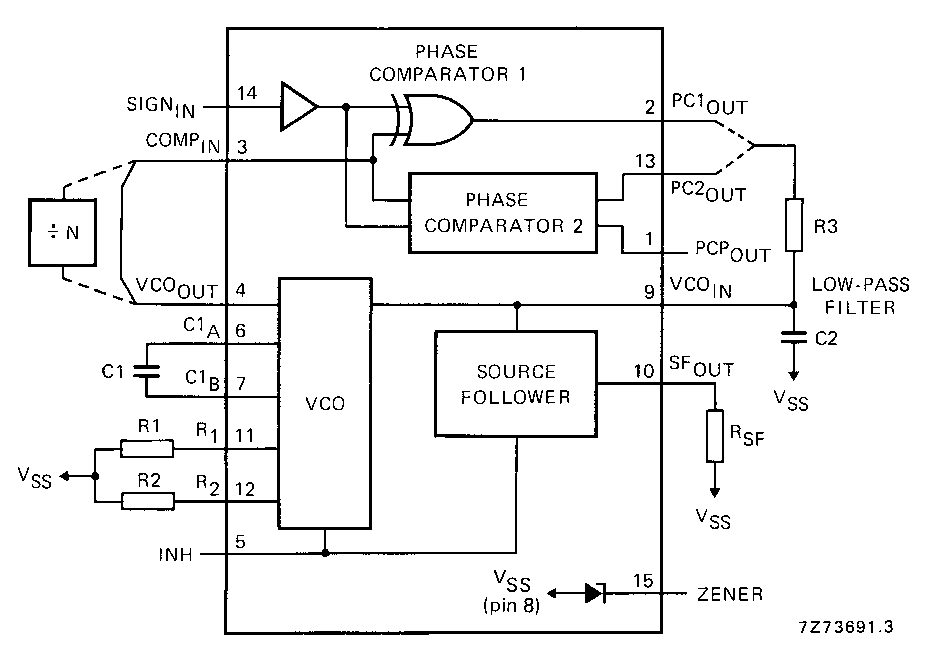
\includegraphics[scale=0.6]{report_img/4046_crop}
	\end{center}
\end{figure}

\section{SA612A Pin Configuration}
\label{app:SA612A}
Pin configuration of the SA612A mixer chip used\cite{SA612A}.
\begin{figure}[h!]
	\begin{center}
		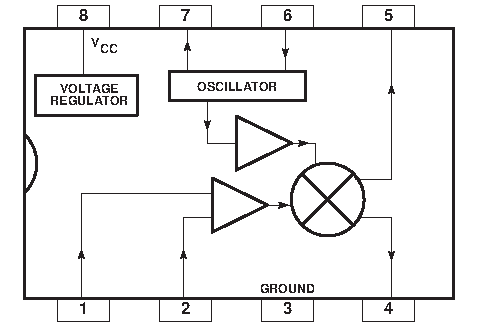
\includegraphics[scale=1]{report_img/SA612A_crop}
	\end{center}
\end{figure}

\section{TL081 Op-Amp}
\label{app:lt081}
Internal structure and pin diagram of the LT081 operational amplifier used in the low pass filter\cite{TL081}.
\begin{figure}[h!]
\centering
\subfigure[Internal circuit diagram.]{
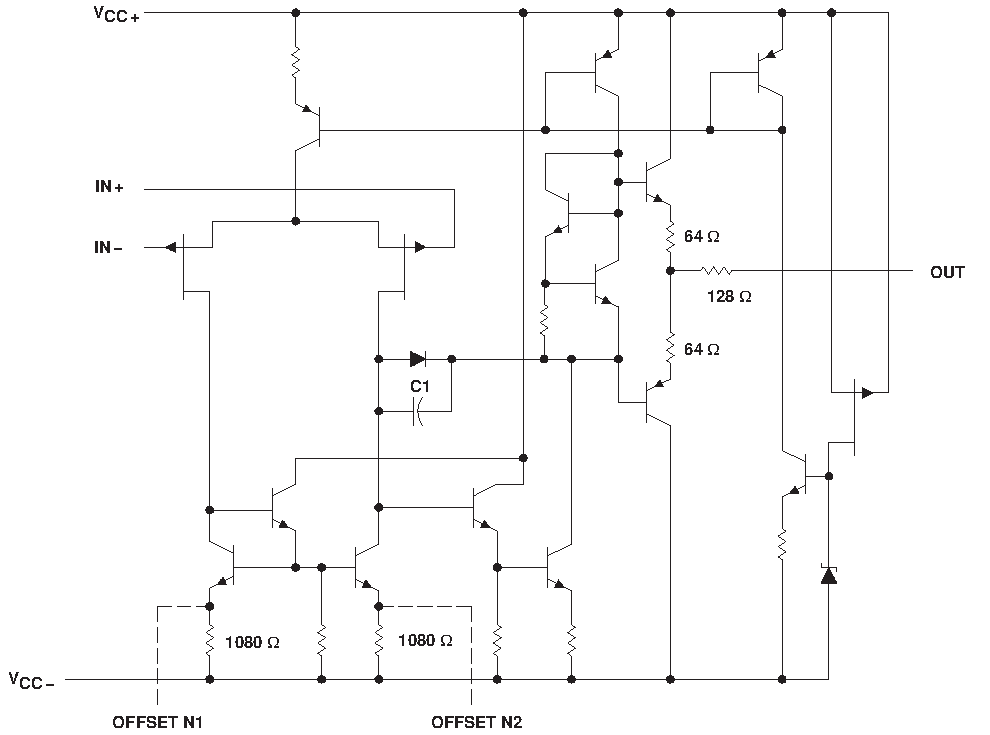
\includegraphics[scale=0.55]{report_img/lt081_crop1}
\label{fig:subfig1}
}
\subfigure[Pin locations]{
\raisebox{3cm}{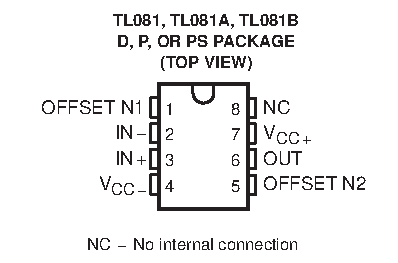
\includegraphics[scale=0.67]{report_img/lt081_crop2}
\label{fig:subfig2}
}}
\label{fig:subfigureExample}
\end{figure}
